\documentclass[tikz,border=8pt]{standalone}
\usepackage{tikz}
\usetikzlibrary{calc}
\begin{document}
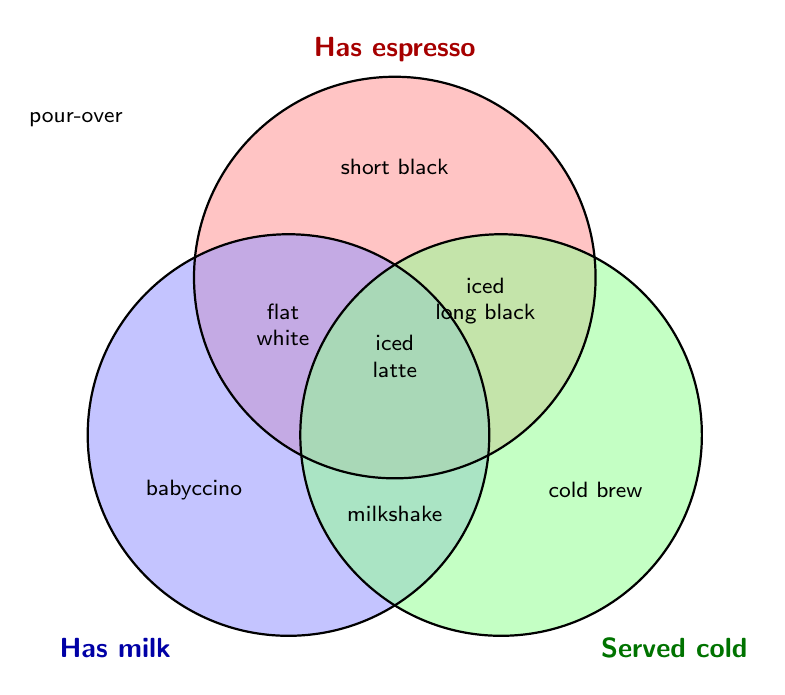
\begin{tikzpicture}[
  font=\sffamily,
  drink/.style={align=center, font=\sffamily\footnotesize, inner sep=0.5pt, text=black},
  setlabel/.style={font=\sffamily\bfseries, align=center}
]

  % Circle centres and radius. Separation is small enough that
  % every pairwise lens and the triple overlap is a clear region.
  \def\R{2.55}
  \coordinate (E) at (0, 1.15);     % Has espresso
  \coordinate (M) at (-1.35,-0.85); % Has milk
  \coordinate (C) at ( 1.35,-0.85); % Served cold

  \fill[red!42,   opacity=0.55] (E) circle (\R);
  \fill[blue!42,  opacity=0.55] (M) circle (\R);
  \fill[green!42, opacity=0.55] (C) circle (\R);
  \draw[thick] (E) circle (\R);
  \draw[thick] (M) circle (\R);
  \draw[thick] (C) circle (\R);

  % Labels outside, colour-matched to their circle.
  \node[setlabel, text=red!65!black]   at (0, 4.05)    {Has espresso};
  \node[setlabel, text=blue!65!black]  at (-3.55,-3.55) {Has milk};
  \node[setlabel, text=green!45!black] at ( 3.55,-3.55) {Served cold};

  % Exclusive regions
  \node[drink] at (0, 2.55)      {short black};   % espresso only
  \node[drink] at (-2.55,-1.55)  {babyccino};     % milk only
  \node[drink] at ( 2.55,-1.55)  {cold brew};     % cold only

  % Pairwise only
  \node[drink] at (-1.42, 0.55) {flat\\white};    % espresso + milk
  \node[drink] at ( 1.15, 0.85)  {iced\\long black}; % espresso + cold
  \node[drink] at ( 0,   -1.85)  {milkshake};     % milk + cold

  % Triple overlap
  \node[drink] at (0, 0.15) {iced\\latte};

  % Complement of all three sets: hot filter coffee, no milk
  \node[drink] at (-4.05, 3.15) {pour-over};

\end{tikzpicture}
\end{document}
